%!TEX root = ../LastNameI-[RnD-MT]Report.tex

\chapter{State of the Art}
\label{SOA}
This chapter assesses the technical knowledge required in understanding classical mechanics and their related fields such as rigid body dynamics. It also aims at providing state of art relating in task specifications in rigid bodies. Further examination state of art for kinematic singularities and some of the decomposition techniques in linear algebra.
\section{Rigid body dynamics}
Rigid body dynamics can be defined as studying motions of systems in chained bodies to which the external forces are applied \cite{paul1979kinematics}. A rigid body system is made of links (rigid bodies) and joints connecting the links together. 
%The rigid bodies can be represented as robot manipulators, kinematic trees which defines these rigid bodies as links which are linked together to other links/rigid bodies by joints. The movement of every joint is with respect to its parent in  the tree. \cite{https://de.mathworks.com/help/robotics/ug/rigid-body-tree-robot-model.html}
The joints acts as motion constraints or as a constraint force to the rigid body, allowing motion in particular directions \cite{featherstone2014rigid}.


The field of dynamics studies or focuses its study on accelerations and forces of rigid bodies. The dynamic algorithms analyze the equations of motion of rigid bodies and allow mathematical calculation for variables in concern. As mentioned above, the equation of motion for general rigid body system gives information about dynamics of that body which can be represented as in \cite{featherstone2014rigid}:
\begin{equation}
I(q)\ddot{q}+ C(q,\dot{q}) = \tau
\label{generaleqnofmotion}
\end{equation}
Where, $I$ represents the inertia matrix in joint space and $q$ is the vector representing position, $\dot{q}$ and $\ddot{q}$ are the vectors representing velocity and acceleration variables respectively, $C$ represents bias force effects of Coriolis and Centrifugal forces along with gravitational and other forces acting on the system in joint space and finally $\tau$ represents the vector of joint forces \cite{featherstone2014rigid}.
\par
In the field of robotics, there are two main dynamics algorithms which are of importance they are forward and inverse dynamics \cite{featherstone2014rigid}.
\begin{itemize}
	\item  \textit{Forward Dynamics} : can be defined as an algorithm which calculates the joint acceleration response when the force/torque is being applied on rigid body ~\cite{featherstone2014rigid}.
	\begin{equation}
	\ddot{q} = FD(model, q, \dot{q},\tau)
	\end{equation}
	\item  \textit{Inverse Dynamics} which can be defined as an algorithm which performs the opposite of forward dynamics, i.e.\ calculates the force/torque which needs to be applied onto the rigid body for the joint acceleration provided ~\cite{featherstone2014rigid}. 
	\begin{equation}
	\tau =  ID(model,q, \dot{q}, \ddot{q})
	\end{equation}
\end{itemize}
%The calculations can be expressed as equations \cite{featherstone2014rigid}:
%\begin{equation}
%\ddot{q} = FD(model, q, \dot{q},\tau)
%\end{equation}
%\begin{equation}
%\tau =  ID(model,q, \dot{q}, \ddot{q})
%\end{equation}
where $FD$ and $ID$ denotes computation of forward dynamics and inverse dynamics respectively. On comparing the above equations to \ref{generaleqnofmotion}, it can be seen that $FD$ and $ID$ can be rewritten as $I^{-1}(q)(\tau - C(q,\dot{q}))$ and $I(q)\ddot{q} + C(q,\dot{q})$ respectively ~\cite{featherstone2014rigid}. Hybrid dynamics can be defined as combination of forward and inverse dynamics operations in which the interest is in calculating the unknown forces and accelerations when there is information about forces/torques at certain joints and the information about joint accelerations at other joints \cite{featherstone2014rigid}. 


The dynamics algorithms can also be used to identify the inertial elements of a rigid body and thus attends the problem of hybrid dynamics as well \cite{featherstone2014rigid}. There are different types of dynamic algorithms are used for finding solutions for problems related to inverse, forward and hybrid dynamics problems. Some of them are:
\begin{enumerate}
	\item \textit{Composite Rigid Body Algorithm} algorithm which computes forward dynamics and joint space inertial matrix of a rigid body \cite{felis2017rbdl}
	\item \textit{Recursive Newton Euler} algorithm and \textit{Lagrangian} formulated algorithm solves for inverse dynamics.
	\item \textit{Articulated-Body Hybrid Dynamics} Algorithm (ABA) ~\cite{featherstone2014rigid}, \textit{Popov-Vereshchagin algorithm} ~\cite{shakhimardanov2015composable} solves problem of hybrid dynamics.
\end{enumerate}	
%In-order to obtain the complete equation of motion, then we need to perform a series of mathematical operations. This can be achieved by starting to collect separate equations of motion for each rigid body and then applying additional motion constraints \cite{featherstone2014rigid}. There are different methods by which can this can be achieved, using the method involving simple dynamic algoithms, method using closed loop systems, other method using only equation of articulated body and the final method is divide and conquer \cite{featherstone2014rigid}.
Constraints can be expressed as an algebraic equation depicting the number of allowed motion directions. They can be classified into equality and inequality constraints \cite{featherstone2014rigid}. They can be further classified into physical and virtual constraints. The physical constraints are the indicated through for example contact with the environment or contact between bodies whereas virtual constraints can be desired motion specified during task specification.\cite{featherstone2014rigid}. The equation of motion of an non-constrained rigid-body system is represented as in \cite{featherstone2014rigid}:
\begin{equation}
I\ddot{q}+C = \tau
\end{equation}
The rigid body system is subjected to motion constraints, then the equation of motion can be represented as in \cite{featherstone2014rigid}
\begin{equation}
I\ddot{q}+C = \tau + \tau_{c}
\end{equation}
where $\tau_{c}$ indicates the constraint force.
%\color{red}"The constraint force delivers zero power along every direction of velocity freedom that is compatible with the motion constraints (Jourdain’s principle of virtual power.)"\cite{featherstone2014rigid} which specifically means that composition of each value of joint velocity and $\tau_{c}$ should be equal to 0 needs to be satisfied.\cite{featherstone2014rigid}\color{black}
%The above constraint equation can be represented mathematically as a linear complementary problem(LCP)\cite{featherstone2014rigid} and also as a quadratic program which will return a basic solution to the equation.\cite{featherstone2014rigid}
%When two rigid bodies come in contact with each other, then they are subjected to contact constraints indicating that the two bodies cannot be penetrated. 
%If φ is a measure of the signed distance between them, meaning that φ < 0 if they overlap, then the contact constraint is given by the inequality φ ≥ 0. The forces that impose this constraint are similarly one-sided: they can act to prevent penetration, but not to prevent separation—they can repel, but not attract. 
%\textbf{Recursive Newton Euler Algorithm}\\
%Inverse Dynamics deals with calculating the force that that must be applied to a rigid body in-turn to produce a given acceleration response. "Inverse dynamics calculations are used in motion control systems, trajectory design and optimization (e.g. for robots and animated figures), in mechanical design, and as a component in some forward dynamics algorithms." \cite{featherstone2014rigid}
%The algorithm calculates the inverse dynamics of a general kinematic tree in precisely three steps.
%
%\begin{itemize}
%	\item Calculation of velocity and acceleration of each body in the tree.
%	\item Calculating the forces that are required to produce these accelerations.
%	\item Calculating the forces that are transmitted across the joints from the forces acting on the bodies.
%\end{itemize}
%
\par
	In real world, currently calculation of dynamics has been adopted different fields such as computer gaming, virtual-reality softwares, in certain simulators also used in animation tools and in different engineering tools \cite{featherstone2014rigid}. Along with the applications there are different softwares which provide the implementations for algorithms of kinematics and dynamics application. Some of them are ODE (Open Dynamics Engine) \cite{rsmith}, Project Chrono which is an Open-Source Physics Engine \cite{ProjectChrono} , ADAMS (Automated Dynamic Analysis of Mechanical Systems) is a software for multi body dynamics simulation \cite{adams}, DART (Dynamic Animation and Robotics Toolkit) \cite{dart}, MuJoCo physics engine \cite{todorov2012mujoco} etc.\ Some of the different softwares made use of are:
\begin{itemize}
	\item KDL (Kinematics and Dynamics Library): This library is used for modeling and computing kinematic chains of robots. It includes implementations of different class libraries for geometrical objects, and also allow specifying motion \cite{kdl}. KDL also includes source code available for inverse and hybrid dynamics algorithms such as Popov Vereschagin hybrid dynamics algorithm and Recursive Newton Euler algorithm. 
	\item RBDL (Rigid Body Dynamics Library): This library contains source code for both forward and inverse dynamics algorithms. They contain Recursive Newton Euler Algorithm (RNEA), Composite Rigid Body Algorithm (CRBA) and Articulated Body Algorithm (ABA) \cite{felis2017rbdl}.
\end{itemize}

\section{Task Specification} 
%In order to deploy the robotic systems into the human environments, we must develop them to be safe and reliable. 
%The developed humanoid robots should be capable of being mobile, manipulable. They should also have ability to perceive and monitor. This induces complexity as the number of degrees of freedom are much more than in conventional industrial robots. This substantial increase in the dimension, contributes to the fundamental problems which is linked with the planning, modeling, programming and controlling. \cite{khatib2004whole}
%In-order to synthesize the whole-body behaviors interactively, multiple behavioral primitives have to be simultaneously controlled, including those that guarantee that the constraints imposed by the robot’s structure and the external environment are satisfied.\cite{SYNTHESIS OF WHOLE-BODY BEHAVIORS THROUGH HIERARCHICAL CONTROL OF BEHAVIORAL PRIMITIVES}.Various movement criteria such as eg. primitives describing the behavior of the center of gravity, the behaviors of the hands, legs, and head, the body attitude and posture, the constrained body parts such as joint-limits and contacts, etc. are controlled by entities such as behavioral primitives. By aggregating multiple primitives, we synthesize whole-body behaviors. For safety and for efficient control, establishing a control hierarchy among behavioral primitives, is exploited to establish control priorities among the different control categories, i.e. constraints, operational tasks, and postures.\cite{SYNTHESIS OF WHOLE-BODY BEHAVIORS THROUGH HIERARCHICAL CONTROL OF BEHAVIORAL PRIMITIVES}
The task specification for redundant robots are not merely specifying pose of a single effector. Instead they might involve specifying task for different end effectors and also involve specifying motion associated with the arms, legs, torso, head etc. There have been different task controlled approaches performed on redundant robots \cite{khatib2004whole}.		
\subsection{Whole Body Operational}
\label{WBS-OCP}
Prior to the whole body operational space control literature (WBOSC) \cite{khatib2004whole} was introduced, the field of robotics focused on operational space formulation (OSF) \cite{khatib1987unified}. The OSF framework applied onto manipulators of rigid body systems control and analyze them by writing control equations at the end effector which account only for forces ~\cite{khatib1987unified}.
The WBOSC is a framework which enables real time control of multiple task primitives related to motion and force of redundant humanoid robots \cite{fok2016controlit}.


In-order to assure the safety of the robot and the environment in which it is deployed, a control hierarchy has been described in which they prioritize the most important constraints over non safety constraints
~\cite{sentis2005synthesis}\cite{khatib2004whole}. They are categorized into three different types of control primitives as in \cite{sentis2006whole}: 
\begin{itemize}
	\item \textit{Constraint handling task}: These primitives (constraints) deal with movements and physical limitations that could harm the robot or the physical environment of the robot. Examples: contacts, avoiding objects/bodies nearby.
	\item \textit{Operational tasks}: These low level primitives deals with manipulation and locomotion, by controlling different parts of robot's body such as feet, hands.
	\item \textit{Posture tasks}: These constraints deal with residual redundancy.
\end{itemize}
%For a humanoid robot, the motion behaviors h ave to be controlled during a whole body task. "There are different ways to achieve the task when taken into consideration that each behavior acts an independent task and also the number of degrees of freedom of the tasks is lesser than the number of joints in the robot".


The control hierarchy indicates that the constraints are taken into consideration as primary tasks and they are never violated, while operational tasks (task primitives and posture primitives) are projected onto the constraint motion null-space. In-order to make use of the additional redundancy i.e with the remaining degrees of freedom, posture primitives are projected into both the null-spaces of constraints and the task. Thus indicating that the posture space of the task consists of all the possible motions which do not interfere the performance of the task \cite{sentis2006whole} \cite{khatib2004whole}.


This hierarchy is used to prevent the secondary constraints from interfering with the primary constraints in the robot’s body.
The prioritization can be visualized as projecting Jacobian into null space of tasks which are given higher priortization. If the Jacobian gets singular, it indicates the that task which is active is ill conditioned, the movement of the robot is not feasible \cite{sentis2006whole}. As mentioned in \cite{sentis2006whole} the higher priority tasks are maintained while removing the control from the task trajectory.

\begin{figure}
	\centering
	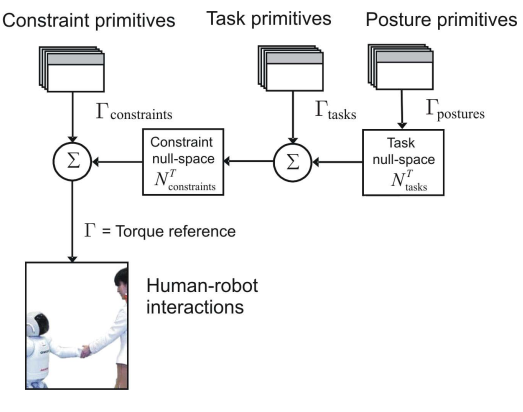
\includegraphics[scale=0.5]{images/OSF}
	\caption{Control scheme representing null space projections \cite{sentis2006whole}}
\end{figure}
The complete joint torque is given by the individual torques are control vectors (operational task, posture task and constraint handling). This is mentioned in the control hierarchy as in \cite{sentis2006whole}:
\begin{equation}
\tau = \tau_{constraints} + N_{constraints}^{T} (\tau_{tasks}+ N_{tasks}^{T}\tau_{posture})
\label{torquescomplete}
\end{equation}


In the above equation $N_{tasks}^{T}$, $N_{constarints}^{T}$ are the matrices representing null space.
%Two tasks are considered in \cite{khatib2004whole}, the first one is called as the primary task and the other is called as the subtask which is controlled within posture space. Initially they perform dynamic modeling of the primary task is performed and later the task/posture decomposition \cite{khatib2004whole} \cite{sentis2005synthesis}\cite{sentis2006whole}.
%\color{black}

%The joint torques are obtained as the result to the computation to the Operational space formulation \cite{vukcevic2018extending}
%The derivation of operational space for building multi level control hierarchy can be given by describing the robot's joint space dynamics. The equation as mentioned in:\cite{sentis2005synthesis}
%\begin{equation}
%I(q)\ddot{q} + C(q,\dot{q}) + g(q) = \tau 
%\end{equation}
%where q represents vector of joint velocities, $I(q)$ is the joint space inertial matrix, C(q, $\dot{q}$) is the generalized bias force namely centrifugal and Coriolis joint forces and g(q) represents the gravitational torque vector and rest if the forces acting on the system , $\tau$ is the vector of joint forces\cite{sentis2005synthesis}.
%
%
Inorder to provide control for the control primitives in different levels of hierarchy, OSF is  described as the decomposition on the level of torques of the desired task (operational task). The torque can be calculated by force transformation \cite{sentis2005synthesis}
\begin{equation}
\tau_{t} = J^{T}_{t}F_{t}
\label{torque}
\end{equation}
Similarly, the joint torques for tasks, constraints and postures described in the equation \ref{torquescomplete} can be represented as in \cite{sentis2005synthesis}:
\begin{equation}
\tau_{tasks} = J_{tasks}^{T}F_{task}
\end{equation}	
\begin{equation}
\tau_{constarints} = J_{constraints}^{T}F_{constarints}
\end{equation}	
\begin{equation}
\tau_{postures} = J_{postures}^{T}F_{postures}
\end{equation}	
$J_{constraints}$, $J_{tasks}$ represent the projections of task space Jacobian onto constraint spaces. $J_{postures}$ represents posture Jacobian which operates in additional redundancy. $F_{constarints}$, $F_{task}$, $F_{postures}$ represents constraint force vectors which control the respective control primitives \cite{sentis2005synthesis}. 
%\begin{equation}
%F_{t} = \Lambda_{t}\ddot{X} + F_{bias,t}
%\end{equation}
%The force can be given by the desired task represented as $\ddot{X}$ and $\Lambda_{t}$ is the inertail matrix in operational space, $F_{bias,t}$ represents the contribution from Coriolis and centrifugal effects and other forces acting on the system.\\
%By substituting in \ref{torque}, the equation can be written as:
%\begin{equation}
%\tau_{t} = J_{t}^{T}(\Lambda\ddot{X} + F_{bias,t})
%\end{equation}
%% This projection prevents the interference of acceleration components onto constrained directions.\cite{sentis2005synthesis}
%%The operational space formulation allows decomposition of torque according to the hierarchy mentioned above, the decoupled vectors are torque concerning the constrained task behavior and the torque concerning the posture space and torque concerning the tasks:\cite{sentis2005synthesis}
%$$\tau = \tau_{constraints} + N_{constraints}^{T} (\tau_{tasks}+ N_{tasks}^{T}\tau_{posture})$$
%The complete joint torque and the individual torques are control vectors (operational task, posture task and constraint handling) as mentioned in the control hierarchy are given as :
%\begin{equation}
%\tau = \tau_{constraints} + N_{constraints}^{T} (\tau_{tasks}+ N_{tasks}^{T}\tau_{posture})
%\label{torquescomplete}
%\end{equation}
%and $N_{tasks}$, $N_{constarints}^{T}$ are the matrices representing null space projections.\cite{sentis2005synthesis}\\
%The joint vectors for tasks, described in the equation \ref{torquescomplete} can be represented as :
%\begin{equation}
%\tau_{tasks} = J_{tasks}^{T}F_{task}
%\end{equation}	
%where $\tau_{p}$ controls the desired torque of the posture. The projection of this vector onto the posture space is given by $N_{t}$
%Thus the final torque decomposition is given by summing up $\tau_{task}$ and $\tau_{posture}$

%As humanoids are required to operate in human environments, efficient manipulation, locomotion skills, and safe contact interactions will be of primary concern.\cite{A Whole-Body Control Framework for Humanoids Operating in Human Environment}.This results in increasing complexity of humanoid mechanisms and their desired capabilities, and hence a crucial need for a generalized framework where a desired whole-body motion behavior can be easily specified and controlled is required.\cite{WHOLE-BODY DYNAMIC BEHAVIOR AND CONTROL OF HUMAN-LIKE ROBOTS}. The framework tries to integrate task-oriented dynamic control and control prioritization allowing to control multiple task primitives while complying with physical and movement-related constraints.\cite{WHOLE-BODY DYNAMIC BEHAVIOR AND CONTROL OF HUMAN-LIKE ROBOTS}.The multiple-task control framework has been prioritized. In-order to synthesize whole-body behaviors interactively, multiple behavioral primitives need to be simultaneously controlled, including those that guarantee that the constraints imposed by the robot’s structure and the external environment are satisfied.\cite{SYNTHESIS OF WHOLE-BODY BEHAVIORS THROUGH HIERARCHICAL CONTROL OF BEHAVIORAL PRIM}.Prioritizing helps in achieving hierarchies between control spaces, in-turn assigning constraint-handling tasks with top priority, while projecting operational tasks in the null space of the constraints, and controlling
%the posture within the residual redundancy.\cite{WHOLE-BODY DYNAMIC BEHAVIOR AND CONTROL OF HUMAN-LIKE ROBOTS}."The operational space formulation provides dynamic models at the task level and structures for decoupled task and posture control. This formulation allows for posture objectives to be controlled without dynamically interfering with the operational task."Achieving higher performance of posture objectives requires precise models of their dynamic behaviors. 

\subsection{Stack of Tasks}
The Stack of Tasks is a control framework which is developed for redundant manipulator control and complex robots like humanoids. The framework supports control based on both kinematic and dynamic descriptions of the robot. Methods based on a hierarchy of tasks (stack of tasks) have motion specification supported for equality and inequality constraints \cite{mansard-icra-12}. 
%In-order to enable to build complex behaviors with robustness and portability properties, the control approaches which are based on task function formalism and particularly are those structured as a prioritized hierarchy of tasks help accomplish. However, in such frameworks, it is difficult to consider a straightforward integration of tasks described by unilateral constraints. Certainly, unilateral constraints exhibit irregularities that prevent the insertion of unilateral tasks at any priority level, other than the lowest, of a hierarchy \cite{A Unified Approach to Integrate Unilateral Constraints in the Stack of Tasks}
%The authors try to generalize the hierarchy-based control schemes to account for unilateral constraints at any priority level. , ( references add) using the operational space formulation\cite{A Unified Approach to Integrate Unilateral Constraints in the Stack of Tasks}. 


Authors in \cite{mansard-icra-12} indicate that, contrarily to WBOSC framework, the tasks use features which can be position of end effector, center of gravity or mass of the robot \cite{stack}. The tasks then can be defined as the difference between desired feature ($s^*$) and the feature based current state of the robot ($s$) as in \cite{mansard-icra-12}: 
\begin{equation}
e = s - s^*
\label{error}
\end{equation}


The above error function depicting the task is regulated to $0$. The components of task can be mapped to both equality or inequality constraints and compute the motion by minimizing the error. Each component representing a task can be \textit{bilateral constraints} or set of represented by inequality constraints. Examples of inequality constraints are singularity and collision avoidances, joint limits etc., \cite{mansard2009unified}.  


The authors Mansard et al., develop their methods which address for task sequencing using Generalized Inverted Kinematics (GIK) \cite{mansard2009versatile} and and then they expand it to task description which uses operational space formulation \cite{escande2014hierarchical,saab2011generation,saab2011generic,mansard2012dedicated,saab2013dynamic}.
The difficulty lies in calculating the desired motion when imposed by the unilateral constraints represented as $e<0$. This is addressed in \cite{mansard2009unified} by various control laws which propose a common activation matrix. The activation matrix is then smoothened at every time step by activating task for each of the inequality constraint values. However, the above approach did not consider the constraints by rigid contacts.


The authors in \cite{saab2011generic} indicate an extension to incorporate modeling of unilateral rigid contacts which can be processed in a generic hierarchal approach using sequence of quadratic programs (QP) which also resolves the equality and inequality constraints. QP is able to take into account two tasks where the first task is developed for equality and inequality constraints. In each of the hierarchical levels the slack constraints are introduced for every task. 


The software framework for controlling redundant robots (SOT) is an open source library with Software Development Kit (SDK) \cite{mansard2009versatile}. This framework is efficiently integrable with CORBA (for communication of systems which have been deployed on different platforms). 


The framework has been developed to compute the value of the feature at the current time instance. The signals indicate the data flow within the system and can be called as input and output signals. The output signal supplies information onto the component called Entity which computes the desired information. The tasks and features are two different classes of entities. There are specific control parameters such as factories of entities, which loads libraries to create, run and destroy entities and a pool is a collection of entities. Some of the other classes of entities are tasks, entities specific for robot dynamic model, entities for walking etc.\ SOT entities use feature entity and compute the task error function (control law) by regulating it \ref{error}.
%The task(e) use features(s). The assumption is made such that the function relates the current state of the robot typically the configuration, speed, acceleration to a feature. Where the function is assumed to be at least differentiable once and the current state of the robot is s(q) and the s* is the desired feature.
%Also each component of a task thus represents a bilateral constraint. On the opposite, there are tasks that would require description through a set of unilateral constraints that are typically represented by inequalities $ei<= 0$.\cite{mansard-icra-12}." The examples of such constraints are joint limits, collision avoidance, visibility loss or avoidance of singularities. 
\subsection{iTaSC}
The original concept of iTASC has been discussed in \cite{smits2008itasc}.
The abbreviated iTASC is called as (Instantaneous Task Specification and Control) \cite{smits2008itasc}. It is a systematic approach which allows to specify constraints on tasks given as relative motions or by allowing dynamic interaction between robot and environment. The constraints can be geometric or dynamic. In general, it can be called as an organized approach to specify constraints for complicated tasks in handling multiple sensor based systems \cite{smits2008itasc}. 
% and  specified in iTASC basically deals with providing a support programmatically for non specalsts to specify complicated tasks in general multiple sensor based robot systems. 


These complicated tasks could be combination of subtasks, feedback from sensors, substantial variety of robot systems, uncertain environments \cite{itasc}. 
%It specifies task in the presence of geometric uncertainities. 
This framework can be applied to many other robotic systems, some of them are mobile robots also to numerous robot systems etc.\ \cite{smits2008itasc}. 
%This framework tries to achieve two major objectives together, one is instantaneously specifying the task and also to obtain estimation in the geometric uncertainity.\cite{smits2008itasc}.
iTASC has certain important advantages over the traditional motion specification methodologies. Firstly, there is no necessity of constraining the complete 6D system and hence constraints can be partially specified. The constraints can be prioritized and these constraints are in-turn instinctively optimize the robot's motion by solving the constrained optimization problem \cite{itascwiki}


In general there are two modeling procedures for the task, one is application independent control and estimation scheme and the other one is 
systematic application dependent task modeling procedure \cite{itasc}.
\begin{figure}
	\centering
	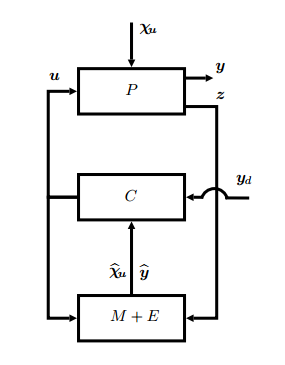
\includegraphics[scale=0.6]{images/iTASC}
	\caption{iTASC control scheme \cite{smits2008itasc}}
	\label{iTASC}
\end{figure}
The \textit{Control and Estimation scheme} is as indicated in the figure \ref{iTASC}. The plant P consists of the main robot system and the environment. The controller is denoted as C, the model update and estimation is denoted as M+E. The control input u to is given to the plant, in robots it is given as joint velocities in velocity scheme ($\dot{q}$). The system output is denoted by y, which is given by controller variables. The reference values to output is given as $y_{d}$. The measurements z is used to observe the plant and the geometric disturbances is given as $X_{u}$ \cite{itasc}\cite{smits2008itasc}. The equations for control system in iTASC is mentioned in \cite{decre2009extending}:


The robot system can be given by the how the changing of joint co-ordinates i.e the state of the robot system is being affected over control input u.  
\begin{equation}
\frac{du}{dt}(q,\dot{q})^{T} = s(q,\dot{q},u)
\end{equation}
The output equation can be represented as a function of joint velocities and feature co-ordinates.
\begin{equation}
y = f(q,X_{f})
\label{outputiTASC}
\end{equation}
By differentiating equation \ref{outputiTASC} w.r.t. time the resulting output equation is obtained in velocity level.
The system output can be imposed with constraints $y_{d}$ on y.
\begin{equation}
y = y_{d}
\label{yd}
\end{equation}
Further differentiating equation \ref{yd} we obtain,
\begin{equation}
\dot{y_{d}} = \dot{y} + K(y_{d} - y)
\end{equation}
where the equation consists of feed forward term and K is the feedback term which compensates for various errors.


The loop closure equation gives the relation between joint velocities, feature co-ordinates and uncertainty co-ordinates.
\begin{equation}
l(q,X_{f},X_{u}) = 0
\end{equation}
By differentiating the above equation w.r.t. time the resulting loop closure equation is obtained in velocity level.



For task modeling iTASC makes use of task co-ordinates. There are two types of task co-ordinates feature co-ordinates ($X_{f}$) and uncertainty co-ordinates ($X_{u}$). The task co-ordinates are usually defined in user defined frames. The end result of using the procedure adopted by this framework allows to chose the frames and task co-ordinates such that the task specification becomes very innate ~\cite{itasc}. The procedure follows by initially identifying the objects and features and also assigning the reference frames. Later on choosing feature co-ordinates which can be a edges, surface, reference frame etc. And every feature is linked to objects which specify relative motions/force between objects. This can be performed by imposing constraints on feature of one object and then similarly on feature of the other object \cite{smits2008itasc}\cite{itasc}.


The authors have extended the framework to support for inequality constraints as well \cite{decre2009extending}\cite{decre2013extending}. They initially validate the approach on non instantaneous tasks. Thus this approach ensures versatility in specifying robot behavior and eases the task adaptations ~\cite{decre2013extending}. 


Equations for generalizing the objective function of the framework's control equation is given as in \cite{decre2009extending}. 
\begin{equation}
 u = r(\mu,\gamma) 
 \label{u}
\end{equation}
where r is denoted as the penalty function for any convex problem defined by user and $\mu$ and $\gamma$ are two objective functions. Even though the convex functions can be solved very robustly, based on the real time requirements the penalty function can be restricted along with the number of constraints    ~\cite{decre2009extending}. Thus equation \ref{u} can be applied for ``instantaneous task specification for velocity based control``, if there are no geometric uncertainties considered, then in general the equation of optimized problem is given as in \cite{decre2013extending}\cite{decre2009extending}:
\begin{equation}
 u = argmin (r(\mu,\gamma_{1},\gamma_{2}))
\end{equation}
which is conditioned to,
$$\frac{du}{dt}(q,\dot{q})^{T} = s(q,\dot{q},u)$$
$$ y = f(q,X_{f}) $$
$$l(q,X_{f}) = 0$$
$$y = y_{d}+\mu$$
$$\frac{d^{i}}{dt^{i}}y \leq  y_{i,max} + \gamma_{1}$$
$$\frac{d^{i}}{dt^{i}}y \geq  y_{i,min} + \gamma_{2}$$
%The constraints are applied limits $y_{i,max}$ and $y_{i,min}$ as lower and upper. \color{red}Here the inequality constraints are stacked for every iteration starting from i, and  are the upper and lower limits on constraints which are applied on $\frac{d^{i}}{dt^{i}}y$ which ensures that the subtasks performed in hierarchy and thus minimizes the error on subsequent subtasks. The authors also mention that the equation[], "contains variables which are all continuous functions of time and thus there are infinite constraints, which is still an ongoing research because the optimization problems are non - convex functions and are strenuous to solve"\cite{decre2009extending}\color{black}
\subsection{ControlIt! framework}
The main objective of \textit{ControlIt!} focuses on general usage of the whole body controller algorithms. It is an open source software framework which addresses the whole body controller algorithms, such that they enable their incorporation onto a substantial system. This framework, can provide its extension to implement on different robot platforms framework, for that reason it requires model description of that robot system URDF, plugin-based modular architecture and also performs addition of new Whole Body Control (WBC) constraints \cite{fok2016controlit}. The authors suggest the need for integrating of the software with external process as there are robot systems like humanoid robots which are highly redundant and contain multi layered software architecture binding the whole body controller. Hence the distributed component software architecture was proposed as they enable the process to run independently as threads ~\cite{fok2016controlit}.


The software architecture of \textit{ControlIt!} acts as the core component in the framework. It is categorized into three groups: configuration software abstractions, whole body control, and hardware abstraction layer. As indicated in the figure \ref{ControlIt} the compound task (tasks prioritized), robot model (computation of kinematic and dynamic properties) and set of constraints are the components of configuration. The WBC forms the binding co-ordinator/manager which brings in other components jointly and acts as servo-loop. While the Hardware Abstraction Layer (HAL) consists of servoclock and robot interface \cite{fok2016controlit} . 


The main principles considered in the development of the software architecture were such that it allowed separation of concerns as mentioned in figure \ref{ControlIt}, platform independent systems (plug-in architecture), reusing the existing software and code, being conscious of considerations during real time and also being able to support software developers who will use this framework and also researchers who can alter this framework \cite{fok2016controlit}.
\begin{figure}
	\centering
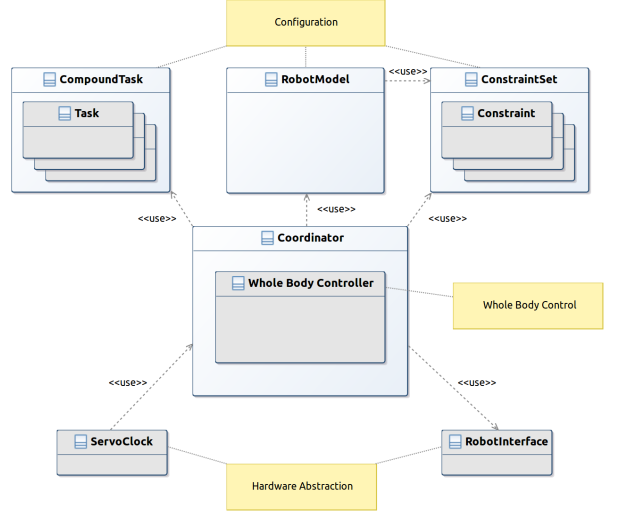
\includegraphics[scale=0.5]{images/controlit_softwarearc}
\caption{Classification of Primary Software Architecture of ControlIt! into three categories \cite{fok2016controlit}}
\label{ControlIt}
\end{figure}
Prior to the implementation of ControlIt, the researchers developed Stanford-WBC \cite{philippsen2011open}, which implemented WBOSC algorithms however did not extend implementation for tree structured robots. Later, UTA-WBC was developed to overcome the disadvantages of Stanford-WBC and was tried on humanoid robot. However, this was developed to certain robot and to those robots behavior specific, and could not assist for common usage of applications \cite{fok2016controlit}. The authors make a comparison between UTA-WBC and ControlIt!, the model library which the ControlIt makes use of is RBDL (Rigid Body Dynamics Library). The current integration of ControlIt is with ROS supports Hydro and Indigo versions also can also simulate on Gazebo platform \cite{vukcevic2018extending}.


The authors from \cite{fok2016controlit} suggest some of the drawbacks that lie in the design of the above framework. The current framework supports only WBOSC based plugins which can be solved analytically. However, there is no support afforded to quadratic programming \cite{escande2014hierarchical} which optimizes inequality constraints. They suggest a future research in identifying if there is possiblity of providing quadratic programming as a plugin to this framework \cite{fok2016controlit}. 
\section{Kinematic Singularities}
There have been analysis of different methods which analyze  and solve the problem of inverse kinematics. Inverse kinematics finds its application in controlling the motions of the rigid body. Inorder to represent inverse kinematics problem , consider a rigid body with links and joints of varied types. Then the joint angles can be represented by a column vector $\theta = (\theta_{1},....,\theta_{k})^{T}$ and the end effector pose can be given by $s = s(\theta)$ indicating they are functions of joint rates. The desired pose for the end effector should reach are indicated by $d = (d_{1},......d_{n})^{T}$ where $d_{i}$ is the position of $i_{th}$ end effector. Thus the IK will find the joint angles for all i such that
\begin{equation}
d_{i} = s_{i}(\theta)
\end{equation}

 
But unfortunately there does not exist any unique solution to this problem. Therefore the Jacobian matrix was introduced as an iterative solution \cite{Buss2004}. This matrix J maps the set of joint angles($\theta$) of the robot to the end effector pose(s).
\begin{equation}
J(\theta) = \frac{\delta s}{\delta \theta}
\end{equation}


The robot reaches kinematic singularity when there is a failure in attaining some of the configurations (i.e.\ joint rates) of the kinematic chain. The mapping between joint and Cartesian spaces are not smooth, i.e.\ a minute change in one of the spaces (giving end effector a samll amount of displacement) will not result in smooth behavioral change in the other space. Mathematically it is indicated by Jacobian matrix being rank deficient as there is a change in the number of motion degrees of freedom \cite{bryunixonline} 
\par
There are mainly two different types of singularity that can occur in the robot they are workspace singularities and internal singularities. The can occur when the arm of the robots are completely stretched or drawn back and the later one could be due to lining up of joint axes \cite{donelan2010kinematic}. The behavior of kinematic chain is different when it reaches singularity. There could be practical effects of singularities in planning a trajectory, the velocity of joints reaching infinity, accuracy in achieving the Cartesian motions etc.\ \cite{bryunixonline}. 
\par
The problem of inverse kinematics can be solved by determining the joint parameters of the robot when the desired position and orientation of the end effector is given \cite{Buss2004}. Few of the most commonly used methods used to solve inverse kinematics include simple analytical methods, iterative/recursive optimizations techniques such as Jacobian transpose methods \cite{balestrino1984robust}, along with heuristic procedure which finds the solution faster and performs cheaper computations such as Cyclic Coordinate Descent \cite{luenberger1984linear}. The manipulators when in singular configuration can be solved as differential equations, presenting solutions to inverse kinematics \cite{siciliano2010robotics}. Some of the other approaches which can be used to detect singularities and to solve the problem of inverse kinematics are numerical methods of SVD, damped least square methods \cite{szkodny2014avoiding}.
\par
The authors in \cite{Buss2004} mention their contribution to the methods which will allow dynamic tracking of end effector to its desired pose which are not reachable. Also the necessity to deal with the unreachable positions arise because the methods such as Jacobian inverse method, pseudo inverse methods will fluctuate greatly. The authors try to elucidate on the mathematical formulations on other methods such as Singular value decompostion(SVD) \cite{de1994singular}, selectively damped least squares (SDLS) \cite{buss2005selectively} \cite{Buss2004}. Another recursive computation method for detecting kinematic singularities in floating space manipulators where the problem is formulated as optimal control theory which is the similar method adopted in the Popov Vereshchagin solver \cite{le2008kinematics}. 
\par
Several measures have been used in order to design the manipulators and determine their pose in working environment, one of them is \textit{manipulability measure} denoted as $J^{T}J$. This quantitative measure determines the ease of moving the manipulator in the Cartesian space but does not have any physical meaning \cite{bryunixonline} \cite{yoshikawa1985dynamic}. By bringing dynamics into consideration, authors in \cite{yoshikawa1985dynamic} introduce \textit{dynamic manipulability measure} which introduces an \textit{weighting matrix}. This allows to match the physical units. Dynamic manipulability measure can be defined as the inertia is felt when it moves in Cartesian space \cite{bryunixonline}. 

%\item A new recursive method that solves the inverse kinematic problem was applied on a free-floating space system with vanishing gravity, for which they compute the joint velocities, given the end-effector velocity.\cite{yoshikawa1985dynamic} The dynamic singularities can occur in such systems, due to the fact that the spacecraft is not fixed as for usual terrestrial manipulators and these singularities cannot be predicted from the knowledge of the system geometric parameters solely.\cite{yoshikawa1985dynamic}. The approach taken by the authors is very new and makes use of a suitable reformulation of the inverse kinematic problem as a multistage optimal control problem, with independent variable the label of the bodies in the chain. The energy conservation property  leads to a purely deductive method for computing the searched after joint velocities.\cite{yoshikawa1985dynamic}
%\end{itemize}
%\section{Limitations of previous work}
\section{Different methods for linear algebra}
\label{algebra}
There are different mathematical decomposition techniques which allow the efficient decomposition/factorization of matrix into simpler components which in-turn ease the complicated matrix operations. Matrix decompositions can be applicable to solve systems of linear equations, or could be based on eigenvalues and concepts related to them and some other decompositions in general. There are certain decomposition techniques and their applications which were looked into and contributed to the mathematical part of the research. 
\subsection{Decomposition and rank one updates}
\begin{itemize}
	\item \textbf{LU Decomposition} : The main applications of this factorization is in determining the inverse of a matrix and also the determinant of the matrix \color{red}\cite{}\color{black} and helps in solving the linear equation or finding solution to the simultaneous linear equation. Also the calculation of determinant of a matrix is easier using this decomposition.
	\item \textbf{Cholesky Decomposition} : This is applicable to positive definite matrices and can be represented as $A = LDL^{T}$ where L is a lower triangular matrix and D represents diagonal elements where there can be non positive entries \cite{higham2009cholesky}. This decomposition is also used to solve linear equations $Ax = b$, where A denotes a symmetric and a positive semi definite matrix. The other advantage is that it requires lesser memory storage \cite{higham2009cholesky}. 
	\item \textbf{SVD} : The main use of this decomposition is that to find a good approximation of low rank matrix which is not trivial. It can also be used for obtaining numerical stability i.e.\ by controlling the condition number which indicates the sensitiveness of the matrix to the variations of input and also rounding errors in the results \cite{sonnberger1989regression}. The other advantages are solving problems relating to linear least square, it is also used in K means clustering for selecting k values, noise filtration, outliers detection in multivariate data etc.\ \cite{slides} 
	\item \textbf{QR Decomposition}: This decomposition is mainly used in finding the eigenvalues of matrix in computer programming languages. This decomposition as all the above solves linear systems, and also to find approximations for least square problems \cite{slides}. A variant of the QR decomposition is RRQR (Rank Revealing QR decomposition) which can be alternative to SVD as it involves detection of rank of a matrix. It is also useful in matrix approximations. Generally RRQR is called as QR decomposition along with column pivoting ~\cite{hong1992rank}
	\item \textbf{UTV Decomposition}: This factorization gives a performance with higher efficiency than SVD. They can be easily updated or downdated. They are also rank revealing like SVD, RRQR. They can also be called as two sided orthogonal decomposition. The implementation for rank one update of UTV decomposition is available in matlab \cite{fierro1999utv}.
	\item \textbf{VSV Decomposition}: These decomposition techniques are also rank revealing like SVD. There have been algorithms which have worked on semi definte matrices and also indefinite matrices which has been discussed in \cite{luk1996symmetric}\cite{baker1998correlation}. When compared to UTV decomposition this decomposition makes use of symmetry in the matrix and thus saves the processing time in computers \cite{fierro2005utv}.
\end{itemize}

\section{Limitations of previous work}
\color{red} write here \color{black}
%allows factorization of matrix into lower and upper triangular matrices along with a permutation matrix.\cite{wikipedia} It can be represented as :\cite{mention from some paper which mentions this} $A = L U$ where L is the lower triangular matrix where all the elements above the diagonal are set to zero and U is the upper triangular matrix which represents that the elements below the diagonal are zero. 
%If matrix A is symmetric and positive definite {appendix} where it can be represented as in the form $A = Y^{T}Y$ "for nonsingular matrix Y".\cite{} In this factorization Y is an upper triangular matrix with diagonal elements to be positive. It is unique and can generally be represented in this form $A = LL^{T}$. Another form of Cholesky decomposition is the LDL factorization. 
%"Cholesky Decomposition is used to solve the system of linear equation Ax=b, where A is real symmetric and positive definite. In regression analysis it could be used to estimate the parameter if XTX is positive definite."taken from slides exact copy paste

%\indent
%Update of matrix through an outer product can be defined as rank one update of a matrix. The representation can be shown as in \cite{Rank One Update And the Google Matrix}
%\begin{equation}
%A^{'} = A + {v}{v}^{T}
%\end{equation}
%The main reason to use rank one updates is that it gives a cheaper and faster matrix inversion.\cite{https://dahtah.wordpress.com/2011/11/29/rank-one-updates-for-faster-matrix-inversion/}. If we already know the inverse of the matrix, then the calculation of the matrix A need not be calculated from the beginning, it can be done by perturbing over $A^{-1}$. The rank one update brings the computational complexity of matrix inverse calculation from $O(n)^{3}$ to $O(n)^{2}$.\cite{https://dahtah.wordpress.com/2011/11/29/rank-one-updates-for-faster-matrix-inversion/}